\subsection{Priprava okolja}
    Sam sem pri programiranju uporabljal operacijski sistem Ubuntu, popularno distribucijo Linuxa, ker je po mojem mnenju programiranje na Linuxu veliko lažje in bolj praktično kot na Windowsih. Tudi programski jezik Python je že prednaložen na večini Linux distribucijah, tako verzija 2.x kot 3.x. Program je napisan v Pythonu verzije 3.5.

    Najprej naložimo knjižnjici, ki jih potrebujemo:

    \inputminted[firstline=1, lastline=2, frame=lines]{bash}{latex/bashscripts.sh}

    Za pisanje kode sem uporabljal odprtokodni program Atom (\texttt{https://atom.io/}), za upravljanje verzij pa program Git, v povezavi z shrambo v oblaku Github (\texttt{www.github.com}). 


\subsection{Pridobivanje podatkov}

    Program od uporabnika pridobi podatke, v katero sliko želi skriti podatke in datoteko s podatki, ki jo želi skriti. Po mojem mnenju je veliko bolje, če lahko v sliko skrijemo katere koli podatke, ne samo besedila. Ko program pridobi ime datoteke, jo odpre kot \texttt{bytes} objekt z imenom \texttt{secret}. 

    \inputminted[firstline=1, lastline=2, frame=lines]{python}{latex/code_parts.py}

    V tem primeru je bolj ``varno'' uporabiti stavek \texttt{with}, saj nam Python samodejno zapre datoteko, ko program konča delo v tistem scopu. Tako ne pride do nenamerne prekomerne porabe spomina, saj imamo datoteko odprto samo toliko časa kot jo res potrebujemo.


\subsection{Pridobivanje gesla}

    Program uporabnika vpraša za geslo, s katerim želi zakriptirati datoteko. Ker v običajnem načinu terminala lahko vidimo, kaj uporabnik vpisuje v terminal, ampak ne želimo, da se vidi tudi geslo, moramo v brezgrafičnem načinu uporabiti posebno Pythonovo knjižnjico \texttt{getpass}.  

    \inputminted[firstline=4, lastline=5, frame=lines]{python}{latex/code_parts.py}

    Ko bo uporabnik vpisoval geslo, se ga ne bo videlo, a bo še vedno spravljeno v spremenljivki geslo. Ker so Pythonove spremenljivke globalno dostopne, je bolje, če gesla ne shranimo v ločeno spremenljivko, saj načeloma lahko nek drug del našega programa dostopa do uporabnikovega gesla. Bolje je če geslo takoj podamo funkciji, ki bo iz gesla naredila \texttt{sha256 hash}.

    \inputminted[firstline=7, lastline=7, frame=lines]{python}{latex/code_parts.py}

    V grafičnem vmesniku \texttt{tkinter} pa objektu \texttt{Entry} dodamo lastnost, da namesto gesla, ki ga vpisuje uporabnik prikaže samo nek znak, v tem primeru \texttt{*}.

    \inputminted[firstline=9, lastline=10, frame=lines]{python}{latex/code_parts.py}

    Ko programu s pritiskom na gumb \texttt{Hide} ali \texttt{Find} povemo, naj med drugim pridobi geslo, ga moramo potem izbrisati iz polja, da ne bi prišlo do kakšne zlorabe gesla.

    \inputminted[firstline=12, lastline=15, frame=lines]{python}{latex/code_parts.py}

    Pythonova funkcija \texttt{del()} izbriše določeno spremenljivko. Za stvari kot so gesla v nizih, je ponavadi bolje, če jih izbrišemo takoj ko jih ne potrebujemo več, namesto da čakamo, da to namesto nas naredi Python.


\subsection{Kriptiranje podatkov}

    Glavni del AES kriptiranja bo za nas opravila knjižnjica \texttt{PyCrypto}, saj je njihova implementacija kriptiranja zagotovo bolj pravilna od takšne, ki bi jo napisal jaz. Sama koda je popolnoma preprosta, vse se zgodi v funkciji \texttt{encrypt(message, key)}, pri čemer je \texttt{message} sporočilo, ki ga želomo zakriptirati, \texttt{key} pa je \texttt{sha256 hash} gesla.

    \inputminted[firstline=17, lastline=19, frame=lines]{python}{latex/code_parts.py}

    Paziti moramo le na to, da je dolžina celotnega sporočila, ki ga želimo zakriptirati z AES algoritmom deljiva z 16. Tudi ustvarjanje hasha je preprosto, saj skoraj vse za nas naredi knjižnjica \texttt{PyCrypto}.

    \inputminted[firstline=21, lastline=23, frame=lines]{python}{latex/code_parts.py}


\subsection{Skrivanje podatkov v sliko}
    Knjižnjica \texttt{PIL} (Pillow) nam omogoča, da s sliko delamo podobno, kot z dvodimenzionalnim seznamom. Najprej ustvarimo novo sliko, in potem za vsako vrstico in vsak stolpec prekopiramo piksel iz originalne slike \texttt{image\_data}. Dokler še nismo skrili celotnega sporočila (\texttt{if index < len(secret):}), vsakemu kanalu na sliki (\texttt{RGBA}) spremenimo zadnja dva bita v vrednost, ki jo potrebujemo.

    \inputminted[firstline=25, lastline=49, frame=lines]{python}{latex/code_parts.py}

    Zato, ker je pikslov v posamezni sliki veliko, uporabimo bitne operacije, ker so malo hitrejše, kot npr. operacije na celih številih. Cela števila si lahko predstavljamo v binarnem zapisu. Če želimo dobiti določene bite nekega števila (v tem primeru vse bite razen zadnjih dveh) uporabimo bitno operacijo and (\texttt{\&}) z enicami na tistih mestih, kjer želimo dobiti bite tistega števila in ničlo na tistih mestih, kjer želimo $0$ v vsakem primeru. Ker želimo dobiti vse bite razen zadnjih dveh, to pomeni, da želimo izvesti operacijo z številom $11111100_{(2)}$ oziroma negiranim številom $0$\ldots$011_{(2)} = 3$. Znak za negacijo v Pythonu pa je \texttt{\~}.

    \inputminted[firstline=51, lastline=51, frame=lines]{python}{latex/code_parts.py}

    Sedaj želimo na zadnji dve mesti, ki sta zagotovo $0$ skriti en bajt naših podatkov, kar pomeni, da bomo v vsako ``barvo'' skrili po dva bita. Če si predstavljamo, da naš bajt izgleda takole: $11001001_{(2)}$ in mi želimo dobiti po dva bita, to izgleda približno tako:

    $$11001001_{(2)} \wedge 00000011_{(2)} = 00000001_{(2)}$$
    $$11001001_{(2)} \wedge 00001100_{(2)} = 00001000_{(2)}$$
    $$11001001_{(2)} \wedge 00110000_{(2)} = 00000000_{(2)}$$
    $$11001001_{(2)} \wedge 11000000_{(2)} = 11000000_{(2)}$$

    Ker želimo te znake dodati na konec barv, moramo dobljena števila spremeniti še z operacijo \texttt{right shift}, v Pythonu \texttt{>>}. Ta operacija vse bite v številu premakne za določeno število v desno.

    $$11011100 \gg 2 = 00110111$$

    Ko naredimo to, samo še z operacijo or (\texttt{|}) dodamo bite barvnim kanalom in vse skupaj shranimo v piksel na novi sliki.

    \inputminted[firstline=53, lastline=53, frame=lines]{python}{latex/code_parts.py}


\subsection{Iskanje podatkov}
    Iskanje podatkov v sliki je precej podobno skrivanju podatkov. Prav tako najprej od uporabnika potrebujemo podatke, v kateri sliki želi iskati podatke, kam bo shranil najdene podatke in geslo. Ena od razlik je, da ko iščemo podatke v sliki, najprej ne vemo, koliko jih je, oziroma do katerega piksla so naši podatki. Zato so v slikah, v katerih so bili skriti podatki s tem programom v prvih 4 pikslih podatki o dolžini, datoteke, ki jo želimo skriti. To pomeni, da je najdaljši možen zapis, ki ga lahko skrijemo v sliko:

    $$(2^8)^4 = 256^4 = 4294967296 > 4 \cdot 10^9$$

    Pri velikosti slik, ki so danes nekaj čez 10 mio pikslov je torej dovolj, da si podatke o dolžini zapomnimo v samo 4 pikslih. 

    \inputminted[firstline=55, lastline=87, frame=lines]{python}{latex/code_parts.py}

    Potem, ko imamo podatke o dolžini skritega sporočila, samo dodajamo najdene podatke na seznam \texttt{secret}. Ko pridobimo vse podatke, pa moramo seznam še dekriptirati in dobimo sporočilo. Ker sporočilo ni nujno samo tekstovno, ga namesto, da bi ga izpisali na zaslonu, shranimo v datoteko, ki jo je poimenoval uporabnik. Zato lahko na ta način v eno sliko lahko skrijemo ne le preprostega besedila, ampak tudi druge dokumente ali celo druge slikovne datoteke.


\subsection{Primer uporabe programa}
    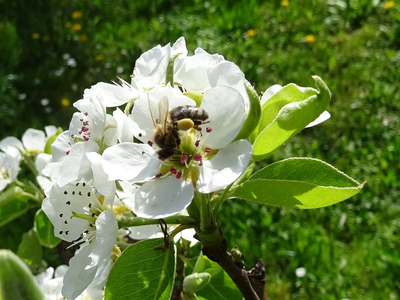
\includegraphics[width=0.5\textwidth]{image.png}
    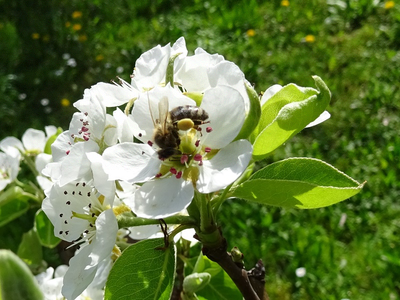
\includegraphics[width=0.5\textwidth]{image_with_hidden_data.png}

    Leva fotografija je samo fotografija čebele na cvetu, velika 400x300 slikovnih točk. Desna slika ji je na prvi pogled enaka, vendar je v njej skrito $10 000$ besed vzorčnega teksta (\textit{Lorem ipsum dolor sit amet\ldots}), zakriptiranih z geslom ``\texttt{geslo}''. Velikost datoteke, ki smo jo skrili je bila 68,1 kB. Prva slika je velika 254,5kB, druga pa 273,3 kB. Sliki se razlikujeta v velikosti, saj zaradi skritih podatkov v najnižjih bitih stiskanje podatkov ni bilo več tako zelo učinkovito. Razlika v velikosti v tem primeru ni bistvena, saj je prva slika že dovolj ``nepravilna'', da že prej ni bilo mogoče slike popolnoma stisniti. Če bi podatke skrivali v sliko, ki bi bila enobarvna, potem bi se velikost spremenila še bolj, poleg tega pa bi bilo s prostim očesom možno opaziti, da je v sliki nekaj skrito (slika ne bi bila več enbarvna, temveč bi bili sosednji piksli med seboj rahlo različnih barv).


    Program lahko uporabljamo na dva različna načina: v grafičnem načinu, ter v načinu ukazne vrstice.

    \subsubsection{Z ukazno vrstico}

        Recimo da imamo datoteko \texttt{slika.png}, v katero želimo skriti naše podatke, ki jih imamo spravljene v datoteki \texttt{skrivnost.txt}. Ime nove slike, v kateri bodo skriti podatki po \texttt{slika2.png}. Program iz ukazne vrstice pokličemo tako:

        \inputminted[firstline=4, lastline=5, frame=lines]{bash}{latex/bashscripts.sh}

        Program nas vpraša za geslo s katerim želimo kriptirati naše podatke, potem pa začne s skrivanjem podatkov v sliko. Ker je slika lahko velika in lahko skrivanje traja nekaj 10 sekund, program sproti prikazuje kako daleč je prišel.

        Če potem želimo najti podatke v sliki z imenom \texttt{slika.png} in jih shraniti v datoteko \texttt{nova\_skrivnost.txt}

        \inputminted[firstline=7, lastline=7, frame=lines]{bash}{latex/bashscripts.sh}

    \subsubsection{Z grafičnim vmesnikom}
        Prav tako je vse mogoče narediti s preprostim grafičnim vmesnikom. Da ga zaženemo, v mapi \texttt{src/} izvedemo naslednji ukaz:

        \inputminted[firstline=9, lastline=9, frame=lines]{bash}{latex/bashscripts.sh}

        Izberemo sliko, v katero želimo skriti podatke, vpišemo geslo za kriptiranje, ime nove slike in datoteko, ki jo želimo skriti. Prav tako lahko s pomočjo grafičnega vmesnika pridobivamo skrite podatke iz slik.

        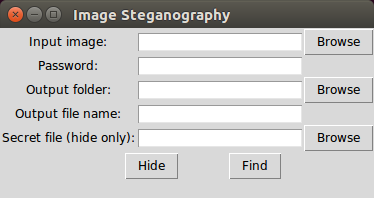
\includegraphics[width=0.6\textwidth]{program_screenshot.png}
